On donne le schéma d’une base de données d’un hôtel.
%\begin{center}
%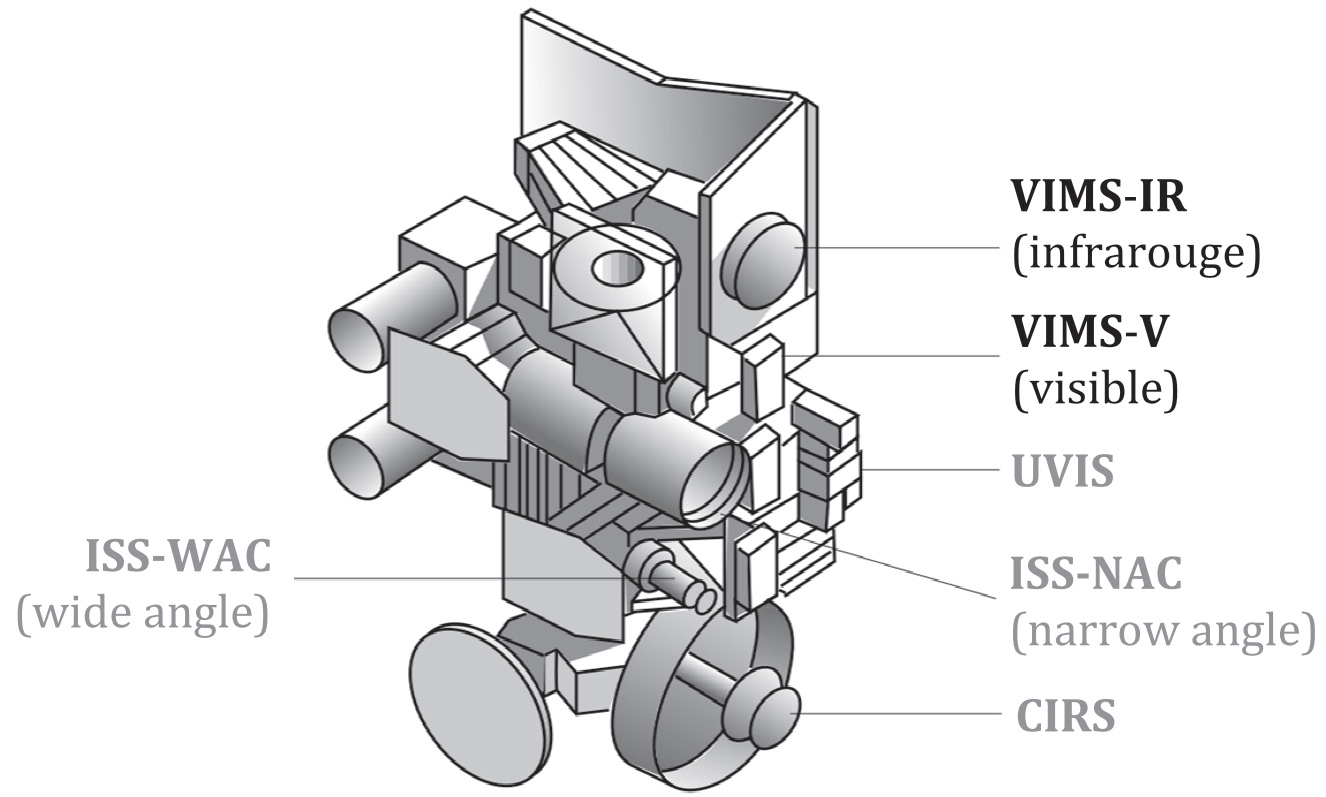
\includegraphics[width=.9\linewidth]{images/fig_01}
%\end{center}

Le modèle physique de la base de données d'un hotel est le suivant.

\begin{center}
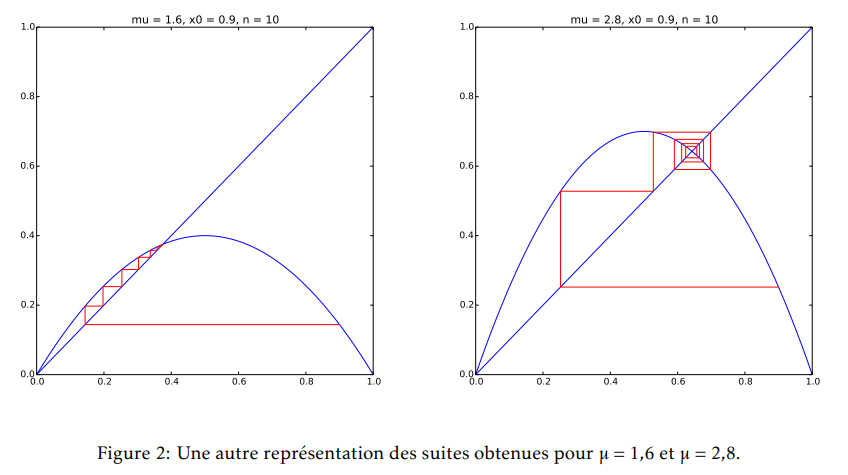
\includegraphics[width=.9\linewidth]{images/fig_02}
\end{center}


La plupart des clefs sont des entiers (I) qui pourront être auto générés par exemple par auto-incrément. Pour certaines entités, notamment celles servant de références à la saisie (\texttt{MODE\_PAIEMENT}, \texttt{TYPE}) la clef est un code. Enfin pour les entités \texttt{TARIF} et \texttt{PLANNING}, il a été choisi une date comme clef. Chaque entité est repérée à l'aide d'un trigramme (code de 3 lettres) qui sert de préfixe pour chaque attribut. Exemple : \texttt{CHB} pour \texttt{CHAMBRE}, \texttt{LIF} pour \texttt{LIGNE\_FACTURE}, etc... Les booléens seront représentés par des valeurs numériques 0 (faux) et 1 (vrai), chaque attribut ayant obligatoirement une valeur par défaut. L'association << occupée >> permet de connaître la réservation ou l'occupation d'une chambre (une chambre peut avoir été réservée mais pas occupée), c'est pourquoi cette association possède les attributs \texttt{NB\_PERS} (nombre de personnes : entier) \texttt{RESERVE} (réservée : booléen) et \texttt{OCCUPE} (occupe : booléen). 

Une chambre à une date donnée, ne peut être occupée que par un seul client. Mais un client peut occuper plusieurs chambres à la même date ou la même chambre à différentes dates, voire même plusieurs chambres à plusieurs dates...


Définition des entités :
\begin{itemize}
\item l'entité \texttt{CLIENT} : un client peut avoir plusieurs adresses, plusieurs numéros de téléphone et plusieurs e-mail. Pour le téléphone, comme pour l'e-mail, l'attribut \texttt{localisation} permet de savoir si le téléphone est situé au domicile, à l'entreprise, etc...
\item l'entité \texttt{TITRE} permet de donner un titre à une personne, parmi les valeurs \texttt{M.} (monsieur), \texttt{Mme.} (madame) et \texttt{Melle.} (mademoiselle);
\item l'entité \texttt{TYPE} permet de connaître le type de téléphone, parmi les valeurs \texttt{TEL} (téléphone), \texttt{FAX} (télécopie) et \texttt{GSM} (portable);
\item l'entité \texttt{MODE\_PAIEMENT} permet de connaître le genre de paiement, parmi les valeurs \texttt{ESP} (espèces), \texttt{CHQ} (chèque), \texttt{CB} (carte bancaire). L'association << payée >> intègre la date du paiement d'une facture.
\end{itemize}

%NOTA : ce modèle est incomplet. Si l'on devait faire figurer l'adresse sur la facture il faudrait choisir une adresse du client. La meilleure façon de régler le problème est de faire glisser la clef du client dans la table des adresses et d'ajouter dans la table facture l'\texttt{ID} de l'adresse choisie pour la facture.
%
%C'est ce que l'on appelle un << lien identifiant >> qui se positionne au niveau du lien entre l'association << domicilié >> et l'entité << adresse >>. On rajoute alors une association entre la facture et l'adresse de cardinalité 0,1.
%
%
%Il permet de faire apparaître les clés primaires et les clés étrangères entre les différentes tables (relations) de la base de données.

\subsection*{Travail demandé}

\question{Donner la requête permettant de lister tous les noms, prénoms et les titres (M. Mme. ou Melle.) des clients.}

\question{Donner le nombre de clients enregistrés dans la base.}

\question{Trouver les noms et prénoms des clients dont le titre est ‘Mme.' (madame).}

\question{Donner les noms , prénoms et les titres (Mme. ou Melle.) des clientes.}

\question{Donner le nombre de clientes.}

\question{Classer par ordre alphabétique les clients de sexe féminin. On ne demande que les noms et les prénoms qui devront être appelés Noms et Prénoms.}

\question{Établir une nouvelle relation (table) faisant apparaître les noms des clients et leurs numéros de téléphone.}

\question{Donner la liste des clients ayant le même nom}

\question{Donner le nombre d'occurrences de chacun de ces noms.}

%\question{Reprendre la question 2 en faisant apparaître une colonne \texttt{Nom}, une colonne \texttt{Prénom} et une colonne \texttt{Sexe} qui renvoie l’indication << homme >> .}


\question{Donner la valeur moyenne des remises en pourcentage et en montant.}

\question{Donner la valeur maximale des remises en pourcentage et en montant.}

\question{Donner les identifiants facture (\texttt{FAC\_ID} que l'on renomera \texttt{fac$\_$id1}) qui ont bénéficié de remise (soit en pourcentage soit en montant).}

\question{Donner les identifiants clients (\texttt{CLI\_ID}) qui ont bénéficié d’une remise (soit en pourcentage soit en montant).}

\question{Donner les identifiants clients (\texttt{CLI\_ID}) qui n'ont pas bénéficié d'une remise.}


\question{Donner le nom et prénom du client qui a le plus bénéficié de remises. Donner le montant de cette remise totale.}

%\question{Donner le nombre de chambres occupées et non réservées le 28 janvier 2001.}
%
%
%
%\question{Donner le nombre de chambre par étage.}
%
%\question{Donner le nombre de chambres occupées par étage le 28 janvier 2001.}
%
%\question{Donner le nombre de chambres libres par étage le 28 janvier 2001.}
%
%\question{Donner le nombre de nuitées pour chaque chambre au cours de l'année 2000 (une nuitée étant une personne passant une nuit dans une chambre. Si deux personnes occupent la même chambre cela fait deux nuitées).}



%%%%Sujet initial
%\question{Trouver les noms et prénoms des clients dont le titre est ‘Mme.' (madame).}
%
%\question{Classer par ordre alphabétique les clients de sexe masculin. On ne demande que les noms et les prénoms qui devront être appelés Noms et Prénoms.}
%
%\question{Donner la liste des clients ayant le même nom ainsi que le nombre d'occurrences de chacun de ces noms.}
%
%%\question{Reprendre la question 2 en faisant apparaître une colonne \texttt{Nom}, une colonne \texttt{Prénom} et une colonne \texttt{Sexe} qui renvoie l’indication << homme >> .}
%
%
%
%
%%\question{Donner les noms et prénoms des clients dont le nom ne commence pas par B.}
%
%\question{Sélectionner les identifiants facture (\texttt{FAC\_ID}) qui n’ont pas bénéficié de remise (soit en pourcentage soit en montant).}
%
%\question{Donner les identifiants clients (\texttt{CLI\_ID}) qui n’ont pas bénéficié d’une remise (soit en pourcentage soit en montant).}
%
%\question{Donner le nom et prénom de ces clients.}
%
%\question{Donner le nombre de chambres occupées et non réservées le 28 janvier 2001.}
%
%\question{Établir une nouvelle relation (table) faisant apparaître les noms des clients et leurs numéros de téléphone.}
%
%\question{Donner le nombre de chambre par étage.}
%
%\question{Donner le nombre de chambres occupées par étage le 28 janvier 2001.}
%
%\question{Donner le nombre de chambres libres par étage le 28 janvier 2001.}
%
%\question{Donner le nombre de nuitées pour chaque chambre au cours de l'année 2000 (une nuitée étant une personne passant une nuit dans une chambre. Si deux personnes occupent la même chambre cela fait deux nuitées).}